\documentclass[a4paper,
fontsize=11pt,
%headings=small,
oneside,
numbers=noperiodatend,
parskip=half-,
bibliography=totoc,
final
]{scrartcl}

\usepackage{synttree}
\usepackage{graphicx}
\setkeys{Gin}{width=.4\textwidth} %default pics size

\graphicspath{{./plots/}}
\usepackage[ngerman]{babel}
\usepackage[T1]{fontenc}
%\usepackage{amsmath}
\usepackage[utf8x]{inputenc}
\usepackage [hyphens]{url}
\usepackage{booktabs} 
\usepackage[left=2.4cm,right=2.4cm,top=2.3cm,bottom=2cm,includeheadfoot]{geometry}
\usepackage{eurosym}
\usepackage{multirow}
\usepackage[ngerman]{varioref}
\setcapindent{1em}
\renewcommand{\labelitemi}{--}
\usepackage{paralist}
\usepackage{pdfpages}
\usepackage{lscape}
\usepackage{float}
\usepackage{acronym}
\usepackage{eurosym}
\usepackage[babel]{csquotes}
\usepackage{longtable,lscape}
\usepackage{mathpazo}
\usepackage[normalem]{ulem} %emphasize weiterhin kursiv
\usepackage[flushmargin,ragged]{footmisc} % left align footnote
\usepackage{ccicons} 
\setcapindent{0pt} % no indentation in captions

%%%% fancy LIBREAS URL color 
\usepackage{xcolor}
\definecolor{libreas}{RGB}{112,0,0}

\usepackage{listings}

\urlstyle{same}  % don't use monospace font for urls

\usepackage[fleqn]{amsmath}

%adjust fontsize for part

\usepackage{sectsty}
\partfont{\large}

%Das BibTeX-Zeichen mit \BibTeX setzen:
\def\symbol#1{\char #1\relax}
\def\bsl{{\tt\symbol{'134}}}
\def\BibTeX{{\rm B\kern-.05em{\sc i\kern-.025em b}\kern-.08em
    T\kern-.1667em\lower.7ex\hbox{E}\kern-.125emX}}

\usepackage{fancyhdr}
\fancyhf{}
\pagestyle{fancyplain}
\fancyhead[R]{\thepage}

% make sure bookmarks are created eventough sections are not numbered!
% uncommend if sections are numbered (bookmarks created by default)
\makeatletter
\renewcommand\@seccntformat[1]{}
\makeatother


\usepackage{hyperxmp}
\usepackage[colorlinks, linkcolor=black,citecolor=black, urlcolor=libreas,
breaklinks= true,bookmarks=true,bookmarksopen=true]{hyperref}
\usepackage{breakurl}

%meta
%meta

\fancyhead[L]{Redaktion LIBREAS\\ %author
LIBREAS. Library Ideas, 35 (2019). % journal, issue, volume.
\href{http://nbn-resolving.de/}
{}} % urn 
% recommended use
%\href{http://nbn-resolving.de/}{\color{black}{urn:nbn:de...}}
\fancyhead[R]{\thepage} %page number
\fancyfoot[L] {\ccLogo \ccAttribution\ \href{https://creativecommons.org/licenses/by/4.0/}{\color{black}Creative Commons BY 4.0}}  %licence
\fancyfoot[R] {ISSN: 1860-7950}

\title{\LARGE{Editorial \#35: Neutralität. Bibliotheken zwischen Pluralität und Propaganda}}% title
\author{Redaktion LIBREAS} % author

\setcounter{page}{1}

\hypersetup{%
      pdftitle={Editorial \#35: Neutralität. Bibliotheken zwischen Pluralität und Propaganda},
      pdfauthor={Redaktion LIBREAS},
      pdfcopyright={CC BY 4.0 International},
      pdfsubject={LIBREAS. Library Ideas, 35 (2019).},
      pdfkeywords={Bibliothek, Neutralität, Neue Rechte, Bibliothekspraxis, Editorial},
      pdflicenseurl={https://creativecommons.org/licenses/by/4.0/},
      pdfcontacturl={http://libreas.eu},
      baseurl={http://libreas.eu},
      pdflang={de},
      pdfmetalang={de}
     }



\date{}
\begin{document}

\maketitle
\thispagestyle{fancyplain} 

%abstracts

%body
Wir alle hier in der LIBREAS-Redaktion haben auch unsere politischen und
gesellschaftlichen Überzeugungen. Nicht alle die gleichen, aber doch in
der Grundtendenz übereinstimmend: für eine offene Gesellschaft, für
Freiheit, für Demokratie, für Humanismus und Menschenrechte, für eine
soziale und auch ökologische Zukunft. Was in den letzten Jahren
passiert, in der Welt und vor allem im DACH-Raum, mit all den
rassistischen, nationalistischen, autoritären Bewegungen, mit den
Wahlerfolgen rechtsextremer Parteien, dem Mainstreaming von
Anti-Feminismus, der Produktion von Hass, der Ausgrenzung von Menschen,
Verschwörungstheorien, und zuletzt auch noch der Verächtlichmachung
politischer Bewegungen junger Menschen durch, well, \enquote{alte weiße
Männer}, hat uns -- nicht nur uns -- immer und immer wieder erschreckt,
besorgt und wütend gemacht. Ist die Welt verrückt geworden? Machen vor
allem alte Generationen die Welt, die EU, die Zukunft kaputt?

Was uns in dieser Atmosphäre auch erschreckte, war die Reaktion einiger
Bibliotheken und bibliothekarischer Publikationen. Waren gerade
Öffentliche Bibliotheken kurz vorher aktiver und wahrnehmbarer Teil der
großen Bewegung gewesen, Menschen, die nach Europa geflohen waren,
willkommen zu heißen und ihnen die Integration zu erleichtern, gab es
auf dem Bibliothekstag 2018 in Berlin eine Podiumsdiskussion, die uns
als Kumulation einer anderen Bewegung im Bibliothekswesen erschien. Sie
hinterließ den Eindruck, als ob Teile des Bibliothekswesens den Ernst
der Lage nicht verstanden hätten. In der Diskussion ging es eigentlich
darum, wie mit den Medien neu-rechter Verlage umzugehen sei. Das ist
keine unwichtige Frage, denn diese Medien existieren und stellen die
Grundfesten jeder humanistischen Überzeugung in Frage -- mit alten
rassistischen und nationalistischen Vorstellungen, aber geupdateter
Sprache und Sprachstrategie. Sollten Bibliotheken sich dazu verhalten
und wenn ja wie? Teile des Podiums schienen sich nicht einmal auf die
Veranstaltung vorbereitet zu haben, so als ob es sich um ein
austauschbares Thema handelte. Bei der anschließenden Diskussion wurde
-- vielleicht im Affekt -- teilweise mit dem Argument, das sei halt
Neutralität, für das Einstellen dieser neu-rechten Bücher in den Bestand
geworben mit dem Verweis darauf, im Sinne einer Serviceeinrichtung, dass
es ja eine Nachfrage für diese Literatur gäbe. Kurz nach dem
Bibliothekstag erschienen dann in verschiedenen bibliothekarischen
Publikationen Beiträge, auch hochrangiger Kolleginnen und Kollegen, die
ebenfalls mit dem Argument einer angeblich der Bibliothek eigenen
\enquote{Neutralität} die Meinung vertraten, solche Medien müssten neben
anderen -- damit auch solchen, die ihnen widersprechen -- in allen
Bibliotheken eingestellt werden. Es wurde damit auf ein Verständnis von
Medien und Informationen zurückgegriffen, das uns absonderlich
apolitisch vorkam -- so, als wäre das alles nur ein Meinungsstreit, bei
dem alle Beteiligten das gleiche Interesse an der Wahrheit hätten, was
bekanntlich nicht der Fall ist, denn es geht hier um Politik, also
Gesellschaftsgestaltung, nicht um die Wahrheit.

Was soll diese \enquote{Neutralität} sein? Wieso hatten wir den
Eindruck, unter diesem Begriff wurden vor allem die Medien der neuen
Rechten in die Bestände eingefügt? (Oder gab es solche Diskussionen in
den letzten Jahren um andere Medien? Medien von Minoritäten,
feministischen Medien, Medien anderer politischer Richtungen?) Warum
schien uns, als würde mit diesem \enquote{Neutralitäts}-Diskurs vor
allem die autoritäre Rechte unterstützt? Weil das gleiche Spiel in den
letzten Jahren in den Medien zu beachten war, wo unter dem Label der
Meinungsfreiheit vor allem die Meinung eines autoritären Teils der
Gesellschaft verstärkt wurde? (Zumal uns auffiel, wer hier vor allem von
\enquote{Neutralität} sprach: Kolleginnen und Kollegen aus der
Mehrheitsgesellschaft, gut situiert, abgesichert. Kolleginnen und
Kollegen aus marginalisierten Gruppen hingegen -- zu denen wir in der
Redaktion ehrlich gesagt nicht gehören, auch wenn wir (noch?) nicht alle
gut situiert sind -- schienen dazu nicht zu reden: Was dachten die sich
eigentlich dazu? Oder sprachen vor allem die, die sich keine Sorgen
machen müssen, was passieren könnte, wenn die neue Rechte die Macht
übernimmt, von Neutralität, während andere sich Sorgen machten?)

\begin{figure}[h!]
\centering
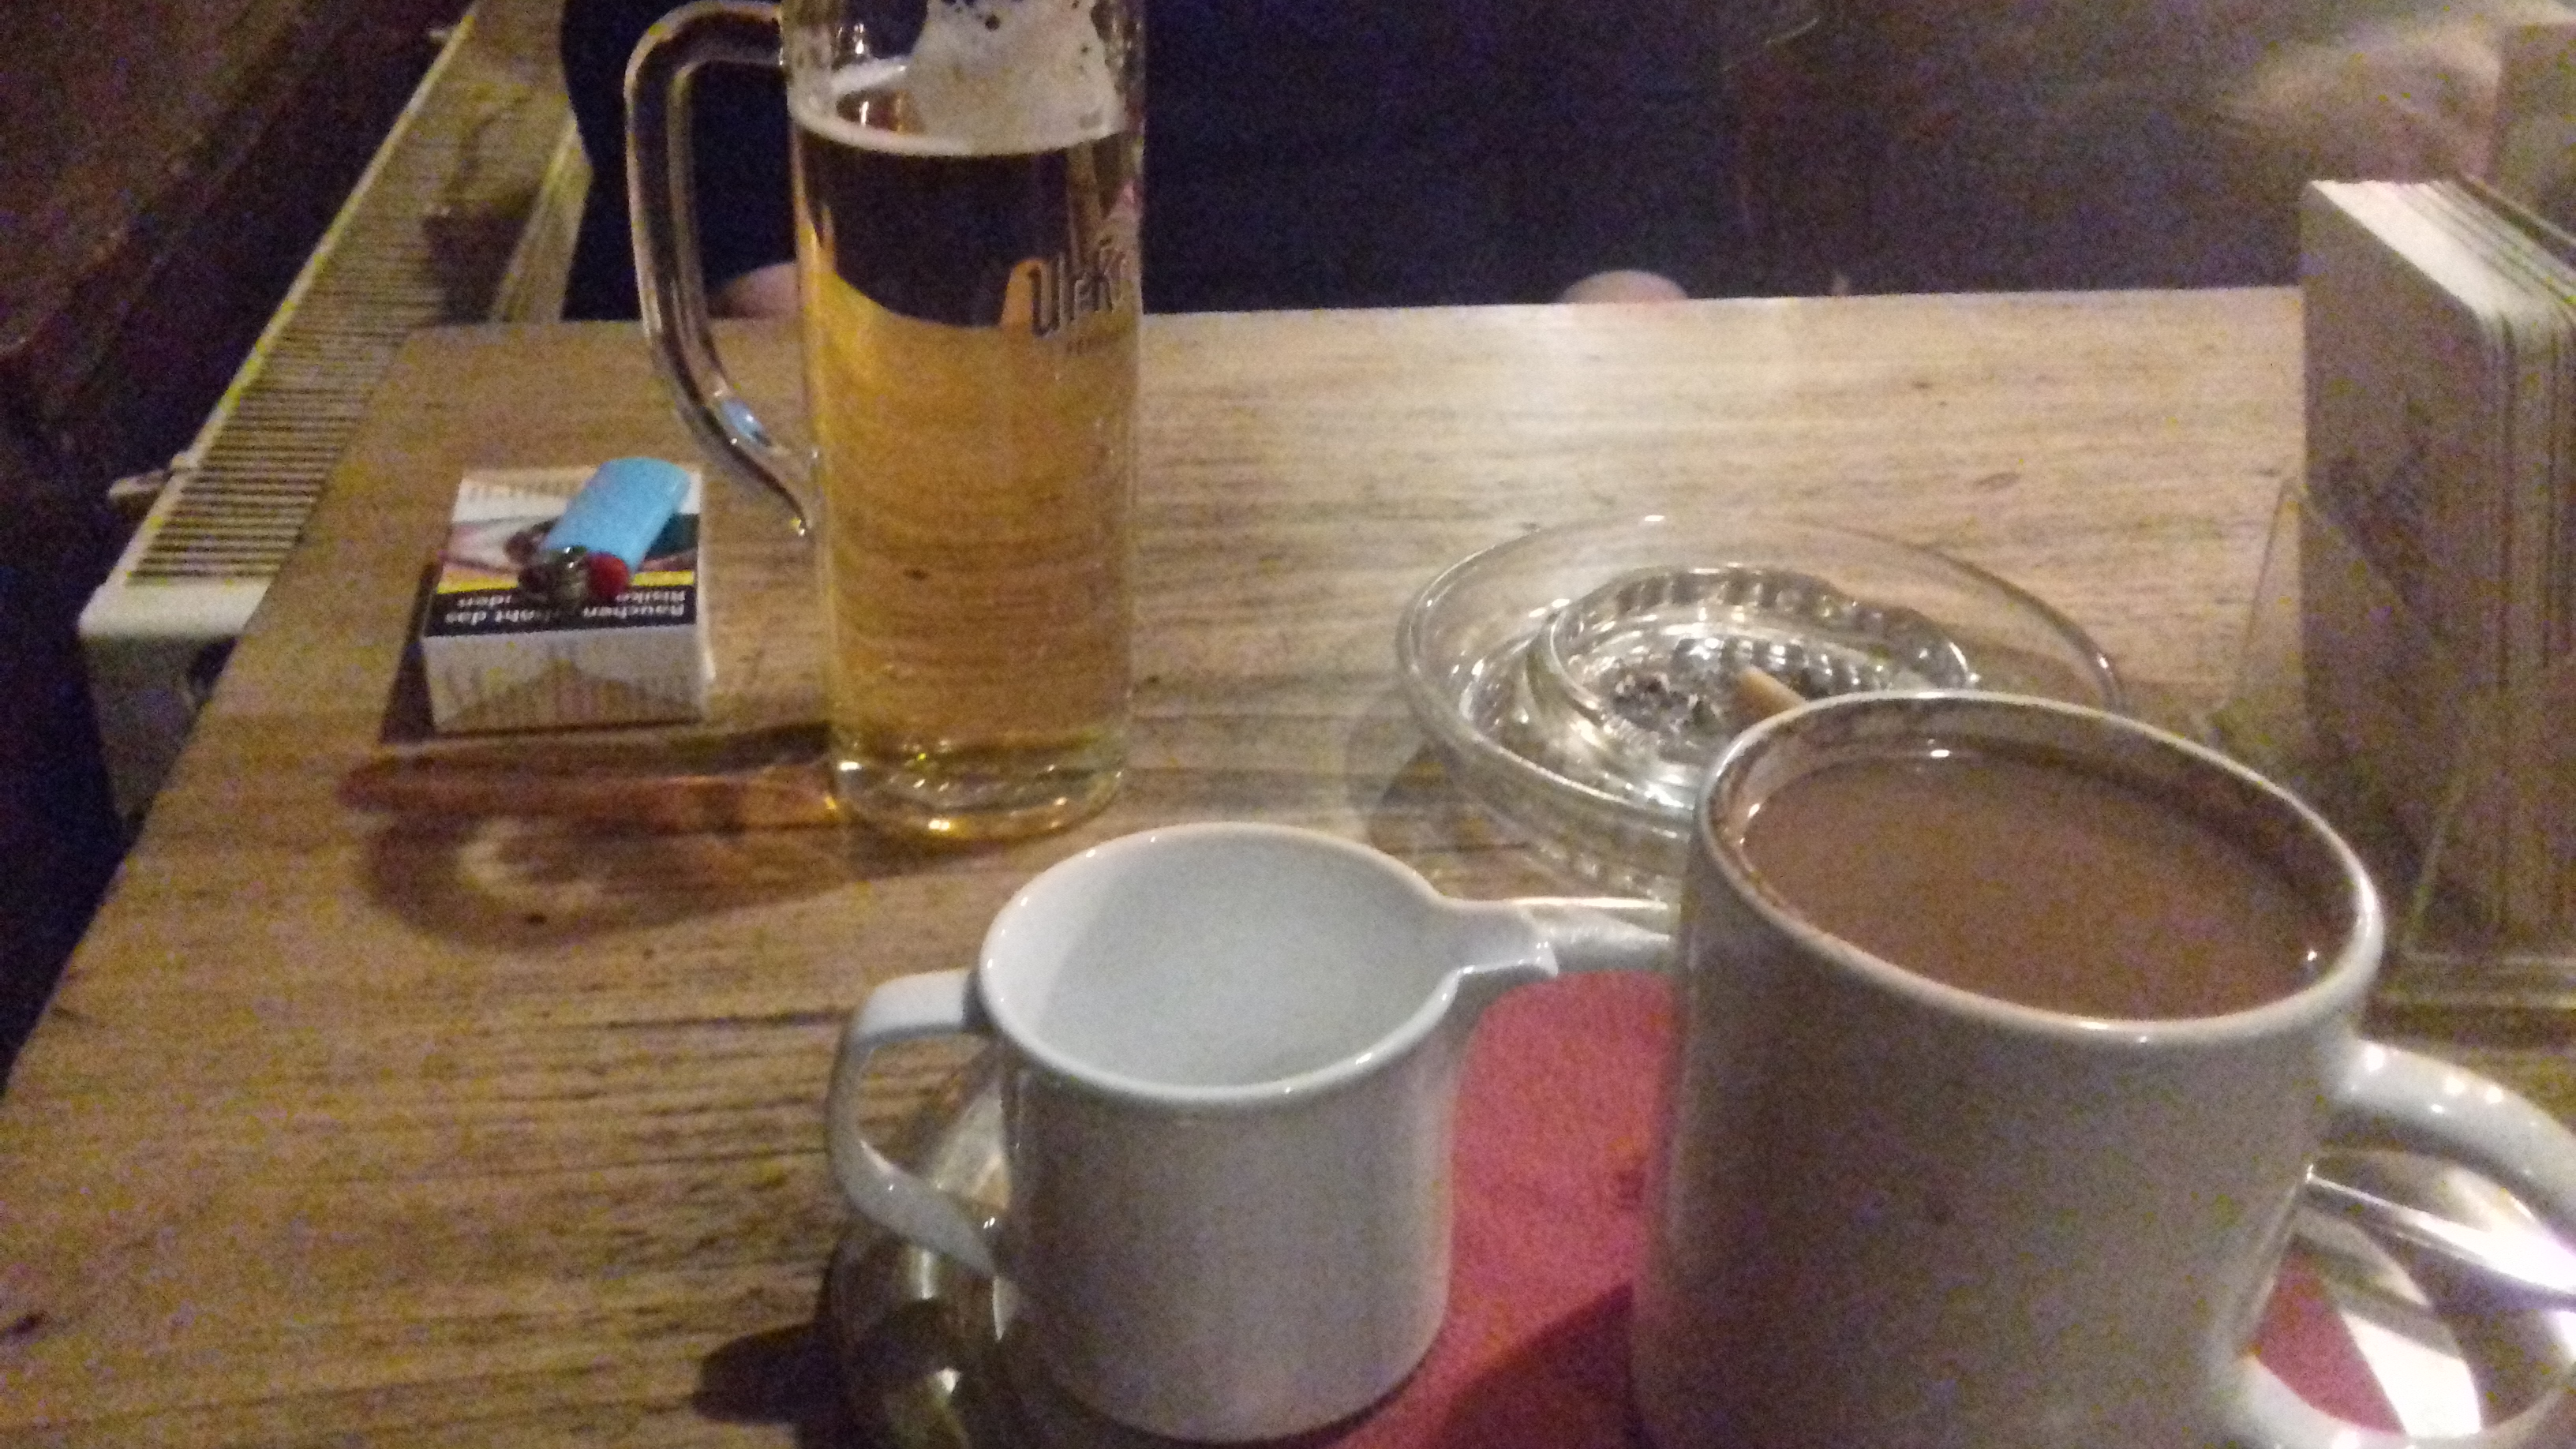
\includegraphics{img/abb.jpg}
\caption{Redaktionsorte XIV. Leipzig-Connewitz, April 2019}
\end{figure}

Uns ist und war das alles nicht geheuer. Deshalb schrieben wir zu diesem
ominösen Begriff der \enquote{Neutralität} -- der auch im
Bibliothekswesen eine Geschichte hat, die aber auch in all den Beiträgen
nicht referiert wird -- einen Schwerpunkt der LIBREAS aus. Wir wollten
wissen, ob wir alleine sind. Wir wollten auch wissen, ob es
differenzierte Überlegungen zu diesem Thema gibt. Hieraus ist die
Ausgabe entstanden.

Wir wissen jetzt, aus den Einreichungen zur Ausgabe und auch aus
Reaktionen auf unseren Call for Papers, dass wir nicht alleine sind mit
unserem Missbehagen an der undifferenzierten Verwendung des Begriffs
\enquote{Neutralität} und auch nicht mit unserem Missbehagen an der
politischen Gesamtsituation. Soviel immerhin. Manchmal ist es wichtig,
sich dessen zu versichern. Es ist nicht so, dass nur wir in der
Redaktion zufällig ähnliche Gedanken haben. \enquote{Wir sind viele}
heißt bekanntlich eine Kampagne von Kultureinrichtungen. Sie gilt
offenbar auch für das Bibliothekswesen.

Während wir diese Ausgabe vorbereiten, gibt es auch bessere Zeichen.
Jugendliche sind, vollkommen zu Recht, für nachvollziehbare Themen auf
der Strasse. Hier und da zeigen Wahlergebnisse wieder in eine andere
Richtung -- in der Türkei, der Slowakei, der Schweiz. Informationen
dazu, wie die neue Rechte redet, wie sie vorgeht, finden immer mehr
Verbreitung. Die neuseeländische Gesellschaft demonstrierte mit ihrer
Reaktion auf das Attentat in Christchurch, dass Gesellschaften auch
heute nicht ins Autoritäre, Rassistische kippen müssen, sondern auch mit
Empathie, Solidarität und klaren Ansagen entgegenhalten können. Der
Generalangriff auf Zukunft, offene Gesellschaft, Menschenrechte,
Demokratie und Fakten scheint nicht so erfolgreich zu sein, wie
befürchtet. Das macht Hoffnung.

Eure / Ihre Redaktion LIBREAS. Library Ideas

(Berlin, Chur, Dresden, Hannover, München)

%autor

\end{document}
